\documentclass[notes,11pt, aspectratio=169]{beamer}

\usepackage{pgfpages}
\setbeameroption{hide notes} % Only slide

\usepackage{array}
\usepackage{tikz}
\usepackage{verbatim}
\setbeamertemplate{note page}{\pagecolor{gray!5}\insertnote}
\usetikzlibrary{positioning}
\usetikzlibrary{snakes}
\usetikzlibrary{calc}
\usetikzlibrary{arrows}
\usetikzlibrary{decorations.markings}
\usetikzlibrary{shapes.misc}
\usetikzlibrary{matrix,shapes,arrows,fit,tikzmark}
\usepackage{amsmath}
\usepackage{mathpazo}
\usepackage{hyperref}
\usepackage{lipsum}
\usepackage{multimedia}
\usepackage{graphicx}
\usepackage{multirow}
\usepackage{dcolumn}
\usepackage{bbm}
\newcolumntype{d}[0]{D{.}{.}{5}}

\usepackage{changepage}
\usepackage{appendixnumberbeamer}

\usepackage[space]{grffile}
\usepackage{booktabs}

% Colors
\definecolor{blue}{RGB}{0,114,178}
\definecolor{red}{RGB}{213,94,0}
\definecolor{yellow}{RGB}{240,228,66}
\definecolor{green}{RGB}{0,158,115}
\definecolor{solutionbg}{RGB}{240,248,240}
\definecolor{solutionframe}{RGB}{0,158,115}

% Solution box environment for worked answers
\usepackage{tcolorbox}
\newtcolorbox{solutionbox}[1][]{
  enhanced,
  colback=solutionbg,
  colframe=solutionframe,
  boxrule=0pt,
  leftrule=3pt,
  arc=0pt,
  left=8pt,
  right=8pt,
  top=6pt,
  bottom=6pt,
  fonttitle=\bfseries,
  title={#1},
  attach boxed title to top left={yshift=-2mm, xshift=5mm},
  boxed title style={colback=solutionframe, colframe=solutionframe, size=small, arc=2pt}
}

\hypersetup{
  colorlinks=false,
  linkbordercolor = {white},
  linkcolor = {blue}
}

\definecolor{MyBackground}{RGB}{255,253,218}

\newenvironment{transitionframe}{
  \setbeamercolor{background canvas}{bg=white}
  \begin{frame}}{
    \end{frame}
}

\setbeamercolor{frametitle}{fg=blue}
\setbeamercolor{title}{fg=black}
\setbeamertemplate{footline}[frame number]
\setbeamertemplate{navigation symbols}{}
\setbeamertemplate{itemize items}{-}
\setbeamercolor{itemize item}{fg=blue}
\setbeamercolor{itemize subitem}{fg=blue}
\setbeamercolor{enumerate item}{fg=blue}
\setbeamercolor{enumerate subitem}{fg=blue}
\setbeamercolor{button}{bg=MyBackground,fg=blue,}

\setbeamercolor{section in toc}{fg=blue}
\setbeamercolor{subsection in toc}{fg=red}
\setbeamersize{text margin left=1em,text margin right=1em}

\newenvironment{wideitemize}{\itemize\addtolength{\itemsep}{10pt}}{\enditemize}
\newenvironment{wideenumerate}{\enumerate\addtolength{\itemsep}{10pt}}{\endenumerate}

\title[]{\textcolor{blue}{ECN 594: Final Review}}
\author[PGP]{}
\institute[FRBNY]{\small{\begin{tabular}{c c c}
Nicholas Vreugdenhil \\
\end{tabular}}}
\date{\today}

\begin{document}

% Title Slide
\begin{frame}
\maketitle
  \centering
\end{frame}

\begin{frame}{Plan}
  \begin{wideenumerate}
    \item \textbf{Part 1 review: Demand and Pricing}
    \item Part 2 review: Competition
    \item Exam logistics
    \item Course wrap-up
  \end{wideenumerate}
\end{frame}

\begin{frame}{Final exam format}
	\begin{wideitemize}
		\item \textbf{Duration:} 80 minutes
		\item \textbf{Allowed:} Calculator + two-sided cheat sheet (letter-size paper)
		\item \textbf{Coverage:} Cumulative (Lectures 1-12)
		\item \textbf{Structure:}
		\begin{wideitemize}
			\vspace{5pt}
			\item Short answer (T/F/NEI, definitions, quick calculations)
			\item Longer problems (derivations, multi-step)
		\end{wideitemize}
		\item Emphasis on Part 2 material, but Part 1 is included
	\end{wideitemize}
\end{frame}

%%%%%%%%%%%%%%%%%%%%%%%%%%%%%%%%%%%%%%%%%%%%%%%%%%%%%%%%%%%%%
% PART 1 REVIEW
%%%%%%%%%%%%%%%%%%%%%%%%%%%%%%%%%%%%%%%%%%%%%%%%%%%%%%%%%%%%%

\begin{frame}{Demand estimation: key concepts}
	\begin{wideitemize}
		\item \textbf{Logit model:} $s_j = \frac{\exp(\delta_j)}{1 + \sum_k \exp(\delta_k)}$
		\item \textbf{Berry inversion:} $\ln(s_j) - \ln(s_0) = \delta_j$
		\item \textbf{Elasticities:}
		\begin{align*}
			\eta_{jj} = \alpha p_j (1 - s_j) \quad \text{(own)} \\
			\eta_{jk} = -\alpha p_k s_k \quad \text{(cross)}
		\end{align*}
		\item \textbf{Consumer surplus:} $CS = \frac{1}{|\alpha|} \ln\left[\sum_j \exp(\delta_j)\right]$
		\item \textbf{IIA problem:} Substitution proportional to share, not similarity
	\end{wideitemize}
\end{frame}

\begin{frame}{T/F: Demand estimation}
	\textbf{True, False, or Not Enough Information?}
	\vspace{8pt}
	\begin{wideenumerate}
		\item In logit, if product A is removed, its share goes disproportionately to similar products.
		\item OLS estimation of $\alpha$ on price is biased toward zero.
		\item The Berry inversion requires data on individual consumer choices.
		\item Consumer surplus from logit depends on the log-sum of $\exp(\delta_j)$.
	\end{wideenumerate}
	\vspace{8pt}
	\centering
	\textit{Take 2 minutes.}
\end{frame}

\begin{frame}{T/F: Demand estimation (solutions)}
	\begin{solutionbox}[Solutions]
		\begin{wideenumerate}
			\item \textbf{FALSE.} IIA: share goes proportionally to market shares, not similarity.
			\item \textbf{TRUE.} High quality $\rightarrow$ high $\xi$ $\rightarrow$ high price; omitted variable bias attenuates $\alpha$.
			\item \textbf{FALSE.} Berry inversion uses market-level shares only, not individual data.
			\item \textbf{TRUE.} $CS = \frac{1}{|\alpha|} \ln\left[\sum_j \exp(\delta_j)\right]$ (the log-sum formula).
		\end{wideenumerate}
	\end{solutionbox}
\end{frame}

\begin{frame}{Identification and IVs}
	\begin{wideitemize}
		\item \textbf{Problem:} $E[p_j \xi_j] \neq 0$ (price endogeneity)
		\item High unobserved quality $\rightarrow$ high price
		\item OLS: $\hat{\alpha}$ biased toward zero
		\item \textbf{Solution:} IVs correlated with $p$, uncorrelated with $\xi$
		\begin{wideitemize}
			\vspace{5pt}
			\item Hausman: prices in other markets
			\item BLP: competitor characteristics
			\item Cost shifters
		\end{wideitemize}
	\end{wideitemize}
\end{frame}

\begin{frame}{Pricing and price discrimination}
	\begin{wideitemize}
		\item \textbf{Lerner index:} $L = \frac{p - MC}{p} = \frac{1}{|\varepsilon|}$
		\item \textbf{Selection by indicators:}
		\begin{wideitemize}
			\vspace{5pt}
			\item Different prices for observable groups
			\item Higher price in more inelastic market
		\end{wideitemize}
		\item \textbf{Two-part tariff:} $F + p \times q$
		\begin{wideitemize}
			\vspace{5pt}
			\item Optimal: $p = MC$, $F = CS$
		\end{wideitemize}
		\item \textbf{Self-selection:} IC binds for high type, IR for low type
	\end{wideitemize}
\end{frame}

\begin{frame}{T/F: Pricing}
	\textbf{True, False, or Not Enough Information?}
	\vspace{8pt}
	\begin{wideenumerate}
		\item With perfect price discrimination, the firm captures all consumer surplus.
		\item A firm using selection by indicators charges higher prices to groups with lower elasticity.
		\item Under optimal two-part tariff, the firm makes zero variable profit.
		\item In self-selection (versioning), the IC constraint binds for the low-type consumer.
	\end{wideenumerate}
	\vspace{8pt}
	\centering
	\textit{Take 2 minutes.}
\end{frame}

\begin{frame}{T/F: Pricing (solutions)}
	\begin{solutionbox}[Solutions]
		\begin{wideenumerate}
			\item \textbf{TRUE.} Perfect price discrimination: firm extracts all surplus.
			\item \textbf{TRUE.} More inelastic $\rightarrow$ higher markup (inverse elasticity rule).
			\item \textbf{TRUE.} Optimal $p = MC$, so variable profit = 0; all profit comes from $F$.
			\item \textbf{FALSE.} IC binds for HIGH type (they might want to pretend to be low type); IR binds for low type.
		\end{wideenumerate}
	\end{solutionbox}
\end{frame}

\begin{frame}{Practice: Consumer surplus calculation}
	\begin{wideitemize}
		\item \textbf{Question:} Logit model with $\alpha = -0.5$. Three products with:
		\begin{wideitemize}
			\vspace{5pt}
			\item $\delta_1 = 2.0$, $\delta_2 = 1.5$, $\delta_3 = 1.0$
		\end{wideitemize}
		\item (a) Calculate total consumer surplus per consumer.
		\item (b) If product 3 is removed, what is the change in CS?
	\end{wideitemize}
	\vspace{10pt}
	\centering
	\textit{Take 4 minutes.}
\end{frame}

\begin{frame}{Practice: Consumer surplus (solution)}
	\begin{solutionbox}[Solution]
		\begin{wideitemize}
			\item \textbf{(a)} $CS = \frac{1}{|\alpha|} \ln\left[1 + \sum_j \exp(\delta_j)\right]$
			\begin{wideitemize}
				\vspace{3pt}
				\item $= \frac{1}{0.5} \ln[1 + e^{2.0} + e^{1.5} + e^{1.0}]$
				\item $= 2 \times \ln[1 + 7.39 + 4.48 + 2.72] = 2 \times \ln(15.59)$
				\item $= 2 \times 2.75 = 5.5$
			\end{wideitemize}
			\item \textbf{(b)} Without product 3:
			\begin{wideitemize}
				\vspace{3pt}
				\item $CS' = 2 \times \ln[1 + 7.39 + 4.48] = 2 \times \ln(12.87) = 5.11$
				\item $\Delta CS = 5.11 - 5.5 = -0.39$
			\end{wideitemize}
			\item Removing product 3 reduces CS by 0.39 per consumer
		\end{wideitemize}
	\end{solutionbox}
\end{frame}

\begin{frame}{Practice: Demand and pricing}
	\begin{wideitemize}
		\item \textbf{Question 1:} Logit model with $\alpha = -0.4$. Product A has $p_A = 30$, $s_A = 0.15$. Calculate the own-price elasticity.
		\item \textbf{Question 2:} Two markets with $\varepsilon_1 = -2$, $\varepsilon_2 = -3$, $MC = 10$. Find optimal prices.
		\item \textbf{Question 3:} A firm uses two-part tariff. Individual demand is $q = 20 - 2p$, $MC = 2$. Find optimal $F$ and $p$.
	\end{wideitemize}
	\vspace{10pt}
	\centering
	\textit{Take 5 minutes.}
\end{frame}

\begin{frame}{Practice: Demand and pricing (solutions)}
	\begin{solutionbox}[Solutions]
		\begin{wideitemize}
			\item \textbf{Q1:} $\eta_{AA} = \alpha p_A (1 - s_A) = (-0.4)(30)(0.85) = -10.2$
			\item \textbf{Q2:} Using $p = \frac{MC}{1 - 1/|\varepsilon|}$:
			\begin{wideitemize}
				\vspace{3pt}
				\item $p_1 = 10/(1 - 0.5) = 20$
				\item $p_2 = 10/(1 - 1/3) = 15$
			\end{wideitemize}
			\item \textbf{Q3:} Optimal $p = MC = 2$. At $p = 2$: $q = 16$.
			\begin{wideitemize}
				\vspace{3pt}
				\item $CS = \frac{1}{2} \times 16 \times 8 = 64$ (triangle)
				\item Optimal $F = 64$
			\end{wideitemize}
		\end{wideitemize}
	\end{solutionbox}
\end{frame}

%%%%%%%%%%%%%%%%%%%%%%%%%%%%%%%%%%%%%%%%%%%%%%%%%%%%%%%%%%%%%
% PART 2 REVIEW
%%%%%%%%%%%%%%%%%%%%%%%%%%%%%%%%%%%%%%%%%%%%%%%%%%%%%%%%%%%%%

\begin{frame}{Plan}
  \begin{wideenumerate}
    \item Part 1 review: Demand and Pricing
    \item \textbf{Part 2 review: Competition}
    \item Exam logistics
    \item Course wrap-up
  \end{wideenumerate}
\end{frame}

\begin{frame}{Oligopoly models}
	\begin{wideitemize}
		\item \textbf{Cournot:} Firms choose quantities
		\begin{wideitemize}
			\vspace{3pt}
			\item Lerner: $L = s_i / |\varepsilon|$
			\item Positive profits
		\end{wideitemize}
		\item \textbf{Bertrand (homogeneous):} $P = MC$, zero profits
		\item \textbf{Hotelling:} $p^* = c + t$ (markup = transport cost)
		\item Cournot applies with capacity constraints
		\item Product differentiation creates pricing power
	\end{wideitemize}
\end{frame}

\begin{frame}{T/F: Oligopoly}
	\textbf{True, False, or Not Enough Information?}
	\vspace{8pt}
	\begin{wideenumerate}
		\item In Cournot, adding more firms always increases total output.
		\item The Bertrand paradox says that two firms are enough for competitive pricing.
		\item In Hotelling with linear transport costs, the equilibrium markup equals the transport cost.
		\item Cournot firms have higher markups when demand is more elastic.
	\end{wideenumerate}
	\vspace{8pt}
	\centering
	\textit{Take 2 minutes.}
\end{frame}

\begin{frame}{T/F: Oligopoly (solutions)}
	\begin{solutionbox}[Solutions]
		\begin{wideenumerate}
			\item \textbf{TRUE.} More firms $\rightarrow$ more competition $\rightarrow$ higher $Q$, lower $P$.
			\item \textbf{TRUE.} With homogeneous products, $N=2$ gives $P=MC$.
			\item \textbf{TRUE.} In symmetric Hotelling: $p^* = c + t$.
			\item \textbf{FALSE.} More elastic demand $\rightarrow$ \textit{lower} markup (from $L = s/|\varepsilon|$).
		\end{wideenumerate}
	\end{solutionbox}
\end{frame}

\begin{frame}{Entry and mergers}
	\begin{wideitemize}
		\item \textbf{Free entry:} $\pi(N^*) \geq F > \pi(N^* + 1)$
		\item \textbf{Entry deterrence:} Requires credible commitment
		\begin{wideitemize}
			\vspace{3pt}
			\item Capacity building
			\item Solve by backward induction (SPE)
		\end{wideitemize}
		\item \textbf{Mergers:} Internalize substitution $\rightarrow$ higher prices
		\item \textbf{Merger simulation:} Change ownership matrix, resolve FOCs
		\item \textbf{HHI:} $= \sum s_i^2 \times 10000$
	\end{wideitemize}
\end{frame}

\begin{frame}{Vertical relationships and collusion}
	\begin{wideitemize}
		\item \textbf{Double marginalization:}
		\begin{wideitemize}
			\vspace{3pt}
			\item Two markups $\rightarrow$ price too high
			\item Solutions: integration, two-part tariff
		\end{wideitemize}
		\item \textbf{Collusion:}
		\begin{wideitemize}
			\vspace{3pt}
			\item $\delta^* = \frac{\pi^D - \pi^C}{\pi^D - \pi^{NE}}$
			\item Cournot: $\delta^* = \frac{(N+1)^2}{N^2 + (N+1)^2}$
			\item Bertrand: $\delta^* = \frac{N-1}{N}$
		\end{wideitemize}
		\item \textbf{Leniency programs:} Create ``race to report''
	\end{wideitemize}
\end{frame}

\begin{frame}{Practice: Entry deterrence}
	\begin{wideitemize}
		\item \textbf{Question:} Monopolist incumbent faces potential entrant.
		\begin{wideitemize}
			\vspace{5pt}
			\item If entrant stays out: Monopolist earns 100
			\item If entrant enters and incumbent accommodates: Both earn 30
			\item If entrant enters and incumbent fights: Both earn $-10$
			\item Entry cost: 20
		\end{wideitemize}
		\item (a) Draw the game tree.
		\item (b) Find the SPE. Will entry occur?
	\end{wideitemize}
	\vspace{8pt}
	\centering
	\textit{Take 4 minutes.}
\end{frame}

\begin{frame}{Practice: Entry deterrence (solution)}
	\begin{solutionbox}[Solution]
		\begin{wideitemize}
			\item \textbf{(a) Game tree:} Entrant moves first (Enter/Stay Out), then Incumbent moves (Accommodate/Fight)
			\item \textbf{(b) SPE by backward induction:}
			\begin{wideitemize}
				\vspace{3pt}
				\item If entry occurs: Incumbent chooses Accommodate (30 $>$ $-10$)
				\item Entrant anticipates: Enter $\rightarrow$ payoff 30 $-$ 20 = 10; Stay Out $\rightarrow$ 0
				\item Entrant enters since $10 > 0$
			\end{wideitemize}
			\item \textbf{SPE:} (Enter, Accommodate)
			\item \textbf{Key insight:} ``Fight'' threat is not credible---incumbent won't follow through
		\end{wideitemize}
	\end{solutionbox}
\end{frame}

\begin{frame}{Practice: Collusion}
	\begin{wideitemize}
		\item \textbf{Question:} Four identical Bertrand firms consider colluding.
		\item (a) What is the minimum discount factor for collusion?
		\item (b) If detection probability is $\rho = 0.2$ and fine is $F = 2\pi^M$, does collusion become easier or harder?
	\end{wideitemize}
	\vspace{10pt}
	\centering
	\textit{Take 4 minutes.}
\end{frame}

\begin{frame}{Practice: Collusion (solution)}
	\begin{solutionbox}[Solution]
		\begin{wideitemize}
			\item \textbf{(a)} Bertrand formula: $\delta^* = \frac{N-1}{N} = \frac{3}{4} = 0.75$
			\item \textbf{(b)} Detection and fines:
			\begin{wideitemize}
				\vspace{3pt}
				\item $\pi^C = \pi^M/4$, $\pi^D = \pi^M$, $\pi^{NE} = 0$
				\item $\rho F = 0.2 \times 2\pi^M = 0.4\pi^M$
				\item $\delta^* = \frac{\pi^D - \pi^C + \rho F}{\pi^D - \pi^{NE} + \rho F}$
				\item $= \frac{\pi^M - 0.25\pi^M + 0.4\pi^M}{\pi^M - 0 + 0.4\pi^M} = \frac{1.15\pi^M}{1.4\pi^M} = 0.82$
			\end{wideitemize}
			\item Higher $\delta^*$ (0.75 $\rightarrow$ 0.82) $\rightarrow$ collusion \textbf{harder}
		\end{wideitemize}
	\end{solutionbox}
\end{frame}

\begin{frame}{Practice: Competition}
	\begin{wideitemize}
		\item \textbf{Question 1:} Cournot duopoly. $P = 120 - Q$, $MC = 20$. Find equilibrium $P$, $Q$, and Lerner index.
		\item \textbf{Question 2:} Market has shares 50\%, 30\%, 20\%. Top two firms merge. Calculate $\Delta HHI$.
		\item \textbf{Question 3:} Bertrand duopoly. What is the minimum $\delta$ for collusion?
	\end{wideitemize}
	\vspace{10pt}
	\centering
	\textit{Take 5 minutes.}
\end{frame}

\begin{frame}{Practice: Competition (solutions)}
	\begin{solutionbox}[Solutions]
		\begin{wideitemize}
			\item \textbf{Q1:} FOC: $120 - 2q_i - q_j = 20$. Symmetric: $q^* = 100/3 \approx 33.3$.
			\begin{wideitemize}
				\vspace{3pt}
				\item $Q = 66.7$, $P = 53.3$
				\item $L = (53.3 - 20)/53.3 = 0.625$ (or $s/|\varepsilon| = 0.5/0.8 = 0.625$)
			\end{wideitemize}
			\item \textbf{Q2:} Shortcut: $\Delta HHI = 2 \times 50 \times 30 = 3000$
			\begin{wideitemize}
				\vspace{3pt}
				\item Pre: $50^2 + 30^2 + 20^2 = 3800$
				\item Post: $80^2 + 20^2 = 6800$
			\end{wideitemize}
			\item \textbf{Q3:} Bertrand with $N = 2$: $\delta^* = \frac{N-1}{N} = \frac{1}{2} = 0.5$
		\end{wideitemize}
	\end{solutionbox}
\end{frame}

\begin{frame}{T/F: Vertical and collusion}
	\textbf{True, False, or Not Enough Information?}
	\vspace{8pt}
	\begin{wideenumerate}
		\item Double marginalization makes the final price too high for both the manufacturer and consumers.
		\item Resale price maintenance is always anticompetitive.
		\item The critical discount factor for Bertrand collusion increases with the number of firms.
		\item Leniency programs help detect cartels by creating a ``race to confess.''
	\end{wideenumerate}
	\vspace{8pt}
	\centering
	\textit{Take 2 minutes.}
\end{frame}

\begin{frame}{T/F: Vertical and collusion (solutions)}
	\begin{solutionbox}[Solutions]
		\begin{wideenumerate}
			\item \textbf{TRUE.} DM hurts manufacturer profits AND raises consumer prices---both sides lose.
			\item \textbf{FALSE.} RPM can be procompetitive (prevents free-riding) or anticompetitive (facilitates collusion).
			\item \textbf{TRUE.} Bertrand: $\delta^* = (N-1)/N$, which increases in $N$.
			\item \textbf{TRUE.} First to report gets immunity $\rightarrow$ Prisoner's Dilemma within cartel.
		\end{wideenumerate}
	\end{solutionbox}
\end{frame}

\begin{frame}{Practice: Double marginalization}
	\begin{wideitemize}
		\item \textbf{Question:} Manufacturer ($MC = 5$) sells to retailer who sells to consumers. Demand: $q = 50 - p$.
		\item (a) Find integrated monopolist's price and profit.
		\item (b) Find prices with vertical separation.
	\end{wideitemize}
	\vspace{10pt}
	\centering
	\textit{Take 4 minutes.}
\end{frame}

\begin{frame}{Practice: Double marginalization (solution)}
	\begin{solutionbox}[Solution]
		\begin{wideitemize}
			\item \textbf{(a) Integrated:}
			\begin{wideitemize}
				\vspace{3pt}
				\item $MR = 50 - 2q = 5 \Rightarrow q = 22.5$, $p = 27.5$
				\item $\pi = (27.5 - 5) \times 22.5 = 506.25$
			\end{wideitemize}
			\item \textbf{(b) Separated:}
			\begin{wideitemize}
				\vspace{3pt}
				\item Retailer: $q = (50 - w)/2$, $p = (50 + w)/2$
				\item Manufacturer: $\max_w (w - 5)(50 - w)/2$
				\item FOC: $w = 27.5$
				\item $p = (50 + 27.5)/2 = 38.75$, $q = 11.25$
			\end{wideitemize}
			\item Price 41\% higher, quantity 50\% lower with separation
		\end{wideitemize}
	\end{solutionbox}
\end{frame}

%%%%%%%%%%%%%%%%%%%%%%%%%%%%%%%%%%%%%%%%%%%%%%%%%%%%%%%%%%%%%
% EXAM LOGISTICS
%%%%%%%%%%%%%%%%%%%%%%%%%%%%%%%%%%%%%%%%%%%%%%%%%%%%%%%%%%%%%

\begin{frame}{Plan}
  \begin{wideenumerate}
    \item Part 1 review: Demand and Pricing
    \item Part 2 review: Competition
    \item \textbf{Exam logistics}
    \item Course wrap-up
  \end{wideenumerate}
\end{frame}

\begin{frame}{What's on the final}
	\begin{wideitemize}
		\item \textbf{Part 1 topics:}
		\begin{wideitemize}
			\vspace{3pt}
			\item Logit, elasticities, IVs, consumer surplus
			\item Lerner index, price discrimination, two-part tariffs
			\item Self-selection (IC/IR)
		\end{wideitemize}
		\item \textbf{Part 2 topics:}
		\begin{wideitemize}
			\vspace{3pt}
			\item Cournot, Bertrand, Hotelling
			\item Entry, entry deterrence
			\item Mergers, HHI, merger simulation
			\item Double marginalization, vertical restraints
			\item Collusion ($\delta^*$ formulas, leniency)
		\end{wideitemize}
	\end{wideitemize}
\end{frame}

\begin{frame}{Comprehensive summary table}
	\begin{center}
		\scriptsize
		\begin{tabular}{|p{2.5cm}|p{4.5cm}|p{4.5cm}|}
			\hline
			\textbf{Topic} & \textbf{Key Formula} & \textbf{Key Insight} \\
			\hline
			Logit & $s_j = \exp(\delta_j)/[1+\Sigma\exp(\delta_k)]$ & IIA: proportional substitution \\
			\hline
			Elasticities & $\eta_{jj} = \alpha p_j(1-s_j)$ & More elastic $\rightarrow$ lower markup \\
			\hline
			Two-part tariff & $p=MC$, $F=CS$ & Extract surplus via fixed fee \\
			\hline
			Cournot & $L = s/|\varepsilon|$ & Positive profits, $\uparrow N \rightarrow \downarrow$ profit \\
			\hline
			Bertrand & $P = MC$ & Zero profits (paradox) \\
			\hline
			Hotelling & $p^* = c + t$ & Differentiation = pricing power \\
			\hline
			Merger & $\Delta HHI = 2s_1 s_2 \times 10000$ & Internalize substitution \\
			\hline
			Collusion & $\delta^* = (\pi^D-\pi^C)/(\pi^D-\pi^{NE})$ & Patient firms can collude \\
			\hline
		\end{tabular}
	\end{center}
\end{frame}

\begin{frame}{Common exam mistakes to avoid}
	\begin{wideenumerate}
		\item \textbf{Confusing IC and IR:} IC binds for HIGH type, IR for LOW type
		\item \textbf{Sign errors on $\alpha$:} $\alpha < 0$, so $|\alpha| = -\alpha$
		\item \textbf{Forgetting $\times 10000$ for HHI:} Shares as percentages
		\item \textbf{SPE vs Nash:} SPE requires backward induction
		\item \textbf{Collusion formulas:} Cournot $\neq$ Bertrand; know both
		\item \textbf{Double marginalization:} Two markups, not one doubled
	\end{wideenumerate}
\end{frame}

\begin{frame}{Key formulas for your cheat sheet}
	\begin{wideitemize}
		\item Logit: $s_j = \exp(\delta_j)/[1 + \Sigma\exp(\delta_k)]$
		\item Berry: $\ln(s_j) - \ln(s_0) = \delta_j$
		\item Elasticities: $\eta_{jj} = \alpha p_j(1-s_j)$, $\eta_{jk} = -\alpha p_k s_k$
		\item Lerner: $L = 1/|\varepsilon|$ (monopoly), $L = s_i/|\varepsilon|$ (Cournot)
		\item HHI: $\Delta = 2 s_1 s_2 \times 10000$
		\item Hotelling: $p^* = c + t$
		\item Collusion: $\delta^* = (\pi^D - \pi^C)/(\pi^D - \pi^{NE})$
	\end{wideitemize}
\end{frame}

\begin{frame}{Final tips}
	\begin{wideenumerate}
		\item Work through practice exam carefully
		\item Review HW1 and HW2 problems
		\item Know the intuition behind formulas, not just formulas
		\item Show your work for partial credit
		\item Manage your time (80 minutes goes fast!)
	\end{wideenumerate}
\end{frame}

\begin{frame}{Time management strategy}
	\begin{wideitemize}
		\item \textbf{80 minutes total} for entire exam
		\item \textbf{Suggested allocation:}
		\begin{wideitemize}
			\vspace{3pt}
			\item Short answer (T/F, definitions): 15-20 minutes
			\item Calculation problems: 15-20 minutes each
			\item Leave 5-10 minutes for review
		\end{wideitemize}
		\item \textbf{If stuck on a problem:}
		\begin{wideitemize}
			\vspace{3pt}
			\item Write what you know (partial credit!)
			\item Move on and come back later
			\item Don't let one question sink you
		\end{wideitemize}
	\end{wideitemize}
\end{frame}

\begin{frame}{Final exam checklist}
	\textbf{Before the exam, make sure you can:}
	\vspace{5pt}
	\begin{wideitemize}
		\item[$\square$] Calculate logit elasticities and consumer surplus
		\item[$\square$] Solve for optimal two-part tariff
		\item[$\square$] Identify when IC vs IR binds in self-selection
		\item[$\square$] Solve Cournot and Bertrand equilibria
		\item[$\square$] Find free entry equilibrium ($N^*$)
		\item[$\square$] Solve entry deterrence games by backward induction
		\item[$\square$] Calculate $\Delta$HHI for mergers
		\item[$\square$] Derive double marginalization prices
		\item[$\square$] Calculate critical discount factors for collusion
	\end{wideitemize}
\end{frame}

%%%%%%%%%%%%%%%%%%%%%%%%%%%%%%%%%%%%%%%%%%%%%%%%%%%%%%%%%%%%%
% COURSE WRAP-UP
%%%%%%%%%%%%%%%%%%%%%%%%%%%%%%%%%%%%%%%%%%%%%%%%%%%%%%%%%%%%%

\begin{frame}{Plan}
  \begin{wideenumerate}
    \item Part 1 review: Demand and Pricing
    \item Part 2 review: Competition
    \item Exam logistics
    \item \textbf{Course wrap-up}
  \end{wideenumerate}
\end{frame}

\begin{frame}{The big picture: what is IO about?}
	\begin{wideitemize}
		\item \textbf{Central question:} When do markets work well, and when do they fail?
		\item \textbf{Our approach:}
		\begin{wideitemize}
			\vspace{5pt}
			\item Estimate demand to understand consumer behavior
			\item Model firm behavior (pricing, entry, competition)
			\item Evaluate policy interventions (mergers, regulation)
		\end{wideitemize}
		\item \textbf{Key insight:} Market power is pervasive---perfect competition is the exception, not the rule
		\item Understanding imperfect competition is essential for business strategy AND public policy
	\end{wideitemize}
\end{frame}

\begin{frame}{How the pieces fit together}
	\begin{center}
		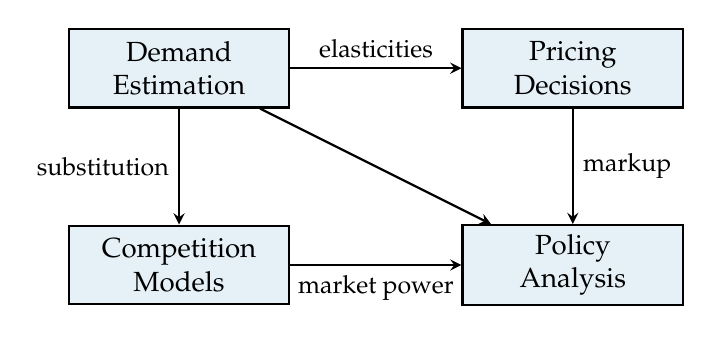
\begin{tikzpicture}[
			box/.style={rectangle, draw, thick, fill=blue!10, minimum width=2.8cm, minimum height=1cm, align=center},
			arrow/.style={->, thick, >=stealth}
		]
			% Boxes
			\node[box] (demand) at (0,2) {Demand\\Estimation};
			\node[box] (pricing) at (5,2) {Pricing\\Decisions};
			\node[box] (competition) at (0,-0.5) {Competition\\Models};
			\node[box] (policy) at (5,-0.5) {Policy\\Analysis};

			% Arrows
			\draw[arrow] (demand) -- node[above, font=\small] {elasticities} (pricing);
			\draw[arrow] (demand) -- node[left, font=\small] {substitution} (competition);
			\draw[arrow] (pricing) -- node[right, font=\small] {markup} (policy);
			\draw[arrow] (competition) -- node[below, font=\small] {market power} (policy);
			\draw[arrow] (demand) -- (policy);
		\end{tikzpicture}
	\end{center}
	\vspace{5pt}
	\begin{wideitemize}
		\item Demand estimation $\rightarrow$ elasticities $\rightarrow$ pricing power
		\item Competition models $\rightarrow$ predict firm behavior
		\item Both feed into policy: merger review, antitrust, regulation
	\end{wideitemize}
\end{frame}

\begin{frame}{The IO economist's toolkit}
	\begin{center}
		\begin{tabular}{|p{4cm}|p{7cm}|}
			\hline
			\textbf{Tool} & \textbf{What it tells us} \\
			\hline
			Logit demand & Consumer preferences, substitution patterns \\
			\hline
			Elasticities & Price sensitivity, competitive pressure \\
			\hline
			Lerner index & Markup, market power \\
			\hline
			Cournot/Bertrand & Oligopoly pricing, profit levels \\
			\hline
			Entry models & Market structure, barriers to entry \\
			\hline
			Merger simulation & Price effects, welfare consequences \\
			\hline
			Collusion theory & Cartel stability, deterrence policy \\
			\hline
		\end{tabular}
	\end{center}
\end{frame}

\begin{frame}{Where IO is used in practice}
	\begin{wideitemize}
		\item \textbf{Antitrust agencies} (DOJ, FTC, EC)
		\begin{wideitemize}
			\vspace{3pt}
			\item Merger review, cartel prosecution
			\item Economic testimony in court cases
		\end{wideitemize}
		\item \textbf{Tech companies} (Amazon, Google, Uber)
		\begin{wideitemize}
			\vspace{3pt}
			\item Pricing algorithms, marketplace design
			\item Demand forecasting, A/B testing
		\end{wideitemize}
		\item \textbf{Consulting firms} (Compass Lexecon, Analysis Group)
		\begin{wideitemize}
			\vspace{3pt}
			\item Litigation support, damages estimation
			\item Regulatory analysis
		\end{wideitemize}
		\item \textbf{Central banks and regulators}
		\begin{wideitemize}
			\vspace{3pt}
			\item Banking competition, consumer protection
		\end{wideitemize}
	\end{wideitemize}
\end{frame}

\begin{frame}{Five things to remember from this course}
	\begin{wideenumerate}
		\item \textbf{Demand matters:} Can't understand markets without understanding consumers
		\item \textbf{Market power is everywhere:} Firms set prices above cost---the question is how much
		\item \textbf{Competition takes many forms:} Cournot, Bertrand, Hotelling capture different realities
		\item \textbf{Structure affects conduct:} Entry, mergers, and vertical relationships shape competition
		\item \textbf{Policy has real effects:} Antitrust, regulation, and leniency programs change outcomes
	\end{wideenumerate}
\end{frame}

%%%%%%%%%%%%%%%%%%%%%%%%%%%%%%%%%%%%%%%%%%%%%%%%%%%%%%%%%%%%%
% KEY POINTS
%%%%%%%%%%%%%%%%%%%%%%%%%%%%%%%%%%%%%%%%%%%%%%%%%%%%%%%%%%%%%

\begin{frame}{Key Points: Part 1}
	\vspace{11pt}
	\begin{wideenumerate}
		\item Logit demand + Berry inversion for estimation
		\item IVs needed: price endogeneity biases $\alpha$ toward zero
		\item IIA problem: demographics partially help
		\item Lerner index: $L = 1/|\varepsilon|$
		\item Two-part tariff: $p = MC$, $F = CS$
		\item Self-selection: IC binds for H, IR binds for L
	\end{wideenumerate}
\end{frame}

\begin{frame}{Key Points: Part 2}
	\vspace{11pt}
	\begin{wideenumerate}
		\item Cournot: $L = s/|\varepsilon|$; Bertrand: $P = MC$
		\item Hotelling: $p^* = c + t$
		\item Free entry until $\pi(N^*) \geq F > \pi(N^*+1)$
		\item Entry deterrence requires credible commitment (SPE)
		\item Merger simulation: change ownership matrix
		\item Double marginalization: two markups hurt everyone
		\item Collusion: $\delta^* = (\pi^D - \pi^C)/(\pi^D - \pi^{NE})$
	\end{wideenumerate}
\end{frame}

\begin{frame}{Good luck on the final!}
	\begin{wideitemize}
		\item Questions before the exam?
	\end{wideitemize}
\end{frame}

\end{document}
